\documentclass[answers]{exam}

%% Language and font encodings
\usepackage[english]{babel}

\usepackage[T1]{fontenc}

%% Sets page size and margins
\usepackage[a4paper,margin=2cm]{geometry}

%% Useful packages
\usepackage{amsmath, hyperref}
\usepackage{graphicx}
\usepackage{paralist, pgfplots}
%\setlength\FrameSep{4pt}






\pdfpagewidth 8.5in
 \pdfpageheight 11in


%General













%Theorem Environments

\begin{document}




	\begin{center}
	\hfill Sandi Xhumari \\ \textbf{$\triangleright$ In-class Activity 4.4-4.5 $\triangleleft$}\\
\end{center}

\textbf{Purpose:} To understand the Fundamental Theorem of Calculus, i.e., what is the relationship between the definite integral (signed area) of the velocity function of a moving object and its position? How can we leverage this relationship to calculate areas under curved functions?  \\

\textbf{Knowledge/Skills and Criteria for Success:} After this activity you should be able to

\begin{enumerate}[A.]
	\item explain in your own words what the Fundamental Theorem of Calculus says
	\item understand the relationship between velocity, position and signed area under velocity function.
	\item graph the position function given the velocity function
	\item 
	\item 
	
\end{enumerate}

\textbf{Task:}


\begin{questions}

\question \textbf{Fundamental Theorem of Calculus.} Write an example illustrating each part by filling the blanks. Let $f(x)$ be continuous on $[a, b]$. We have

\begin{enumerate}[(1)]
	
	\item $F(x) = \int_{a}^x f(t) dt$ is an antiderivative of $f(x)$. In other words
	\[ F'(x) = \frac{d}{dx}\left( \int_{a}^x f(t) dt \right) = f(x). \]
	

	\hfill \break
$f(t) =$ \hspace{0.5in} $a = $ \hspace{0.2 in} $b = $ \hspace{0.2in} $F(x) = $ \hspace{1.5in} $F'(x) = $ \hspace{0.5in} $F'(3) = $
	\hfill \break
	
	\item If $G(x)$ is \emph{any} antiderivative of $f(x)$ (i.e., a function such that $G'(x) = f(x)$), then $G(x) = F(x) + C = \int_{a}^x f(t) dt + C$ and 
	\[ \int_{a}^b f(t) dt = G(b) - G(a) =: G(x)\bigg\rvert_a^b\]


\hfill \break
$G(x)= $ \hspace{1in} $\displaystyle \int_{a}^b f(t) dt = $
\hfill \break

\end{enumerate}

\question Suppose $f(x)$ is differentiable. Then $\displaystyle \int_0^x f'(t) dt = f(x)$ is

\begin{enumerate}[(a)]
	
	\item Always true
	
	\item Sometimes true
	
	\item Never true
	
\end{enumerate}






\question Let $\displaystyle F(x) = \int_{-5}^x t^2+\sin(t) dt$. Find the following.


\begin{enumerate}[(a)]
	
	\item $F(-5) = $
	
	\hfill \break
	
	\item $F\rq{}(x) = $
	
	\hfill \break

	\item $F\rq{}(\pi) = $
	
	\hfill \break
		
	\item $\displaystyle \frac{d}{dx}\left(F(\sin(x))\right) = $
	
	\hfill \break
	
	\item $\frac{d}{dx}\left(\int_{\ln(x)}^{\sin(x)} t^2+\sin(t) dt \right) = $
	
	\hfill \break
	\hfill \break
	\hfill \break
	\hfill \break
	
	\item $F(1) = $
	
	\hfill \break
	\hfill \break
	\hfill \break
	\hfill \break
	
\end{enumerate}

\question Let $v(t)$ be the velocity of a particle moving in a straight path on $[0,6]$. Assume that the position $S(t)$ of the particle was 0 units at the start, i.e., $S(0) = 0$.

\begin{center}
	
	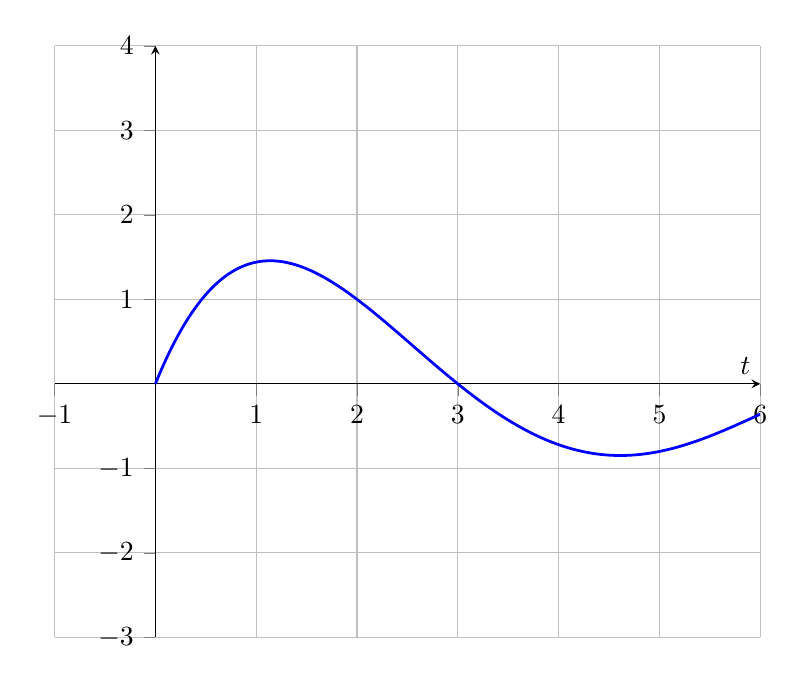
\begin{tikzpicture}
	
	\begin{axis}[xmin=-1,
	xmax=6,
	ymin=-3,
	ymax=4,
	width=300pt,
	xlabel=$t$,
	%ylabel={$f(t)$},
	axis x line=middle,
	axis y line=center,
	tick align=outside,
	grid=major]
	
	\addplot[domain=0:6,
	line width=1pt,
	no markers,
	solid,
	blue, samples=500] {-x*(x-3)*(x-7)^2/50};	
	
	
	
	\end{axis}
	
	\end{tikzpicture}
	
\end{center}

\begin{enumerate}[(a)]
	
		
	\item At what time was the particle the furthest away from the starting point? How far is that approximately?
	
	\hfill \break
	\hfill \break
	\hfill \break
	
	
	\item Describe when is $S(t)$ increasing, decreasing, concave up, or concave down on the interval $[0,6]$.
	
	\hfill \break
	\hfill \break
	\hfill \break
	
	\item Sketch the graph of $S(t)$ on the interval $[0,6]$ in on the same picture above. 
	
	
\end{enumerate}

\question Graph $f(t) = -t^2+4$ on $[0, 2]$. Let $g(x) = \int_0^x f(t) dt$. Then for $x$ on $(0, 2)$, $g(x)$ is 

\begin{enumerate}[(a)]
	
	\item increasing and concave up.
	
	
	\item increasing and concave down.
	
	\item decreasing and concave up.
	
	\item decreasing and concave down.
	
	
\end{enumerate}

\question Please write below any feedback you would like to share about this handout. If you found any parts confusing due to wording or anything like that, please suggest fixes. Thank you!

%\newpage
%
%\question The velocity of an object moving straight up/down under the acceleration of gravity is given as $v(t) = -32t+48$, where time $t$ is given in seconds and velocity is in ft/s. When $t = 0$, the object had a height of $0$ ft. 
%
%\begin{enumerate}[(a)]
%	\item What was the initial velocity of the object?
%	
%	\hfill \break
%	\hfill \break
%	
%	\item What was the maximum height of the object?
%	
%	
%	\hfill \break
%	\hfill \break
%	\hfill \break
%	\hfill \break
%	\hfill \break
%	\hfill \break
%	\hfill \break
%	\hfill \break
%	\hfill \break
%	
%	
%	
%	\item What was the height of the object at time $t = 2$?
%	
%	\hfill \break
%	\hfill \break
%	\hfill \break
%	
%	\item What is the position function $S(t)$ of this object?
%	
%	\hfill \break
%	\hfill \break
%	
%\end{enumerate}



\end{questions}



\end{document}